\documentclass{article}
\usepackage[T1]{fontenc}
\usepackage{lmodern}
\usepackage{graphicx}
\usepackage{amsmath,amssymb}
\usepackage[a4paper,margin=2cm]{geometry}
\usepackage[absolute,overlay]{textpos}
\setlength{\TPHorizModule}{1mm}
\setlength{\TPVertModule}{1mm}
\usepackage[indonesian]{babel}
\usepackage{hyperref}
\setlength{\emergencystretch}{2em}
% unit: Halaman 92

\begin{document}

% === Halaman 92 (llm) ===

3. Column round dan diagonal round

// Column round

\vspace{99.20mm}

\begin{align*}
QR(0, 4, 8, 12) & \quad // \text{ kolom 1} \\
QR(1, 5, 9, 13) & \quad // \text{ kolom 2} \\
QR(2, 6, 10, 14) & \quad // \text{ kolom 3} \\
QR(3, 7, 11, 15) & \quad // \text{ kolom 4}
\end{align*}

\vspace{10mm}

// Diagonal round

\begin{align*}
QR(0, 5, 10, 15) & \quad // \text{ diagonal 1} \\
QR(1, 6, 11, 12) & \quad // \text{ diagonal 2} \\
QR(2, 7, 8, 13) & \quad // \text{ diagonal 3} \\
QR(3, 4, 9, 14) & \quad // \text{ diagonal 4}
\end{align*}

% deskripsi: Tabel 4x4 berisi angka 0 sampai 15 yang menunjukkan indeks posisi elemen untuk proses Column round dan Diagonal round.
% bbox normalisasi: [0.5960, 0.2860, 0.7600, 0.6200]
\begin{textblock*}{34.44mm}(125.16mm,84.94mm)
\noindent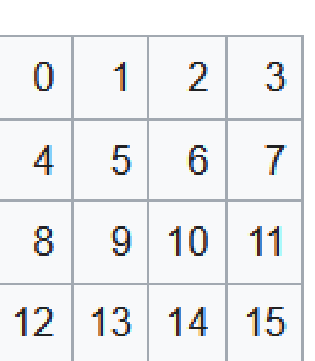
\includegraphics[width=34.44mm,height=99.20mm]{../../images/llm/page_092_img_01.png}%
\end{textblock*}

\end{document}
